\section{Testing}
The scenario used for testing is the one shown in figure \ref{fig:threestationsetup}.\\
Each station sends a message that looks like this:\\
%\begin{align}
%$packet = "S to R"$
%$S = station ID of the center (ThisStation)$
%$R = station ID of the receiver (neighbours[receiver].stationID)$
%\end{align}

%\begin{comment}
\begin{align*}
  E(R_{i,t})    &= E(\alpha_i)+E(\beta_{i,F_1 } F_{1,t})+E(\beta_{i,F_2 } F_{2,t})+\ldots+E(\beta_{i,F_m } F_{m,t}) \\
  \bar{R}_{i,t} &= a+\hat{\beta}_{i,F_1 } E(F_{1,t})+\hat{\beta}_{i,F_2 } E(F_{2,t})+\ldots+\hat{\beta}_{i,F_m } E(F_{m,t}) \\
  \bar{R}_{i,t} &= a+\gamma_1\hat{\beta}_{i,F_1 } +\gamma_2\hat{\beta}_{i,F_2 } F_{2,t}+\ldots+\gamma_m\hat{\beta}_{i,F_m }
\end{align*}
%\end{comment}

\begin{align*}
Packet &= S to R\\
S &= ThisStation\\
R &= neighbours[receiver].stationID
\end{align*}

Where Packet is the packet that is sent to the receiver, S is the station ID of the sending station and R is the station ID of the receiving station.\\
For example, for station 1 sending to station 3: $1\ to\ 3$\\
\\~
Screenshot of testing this for three stations, where all stations sends one message to each of the other two:
\begin{figure}[H]
\centering
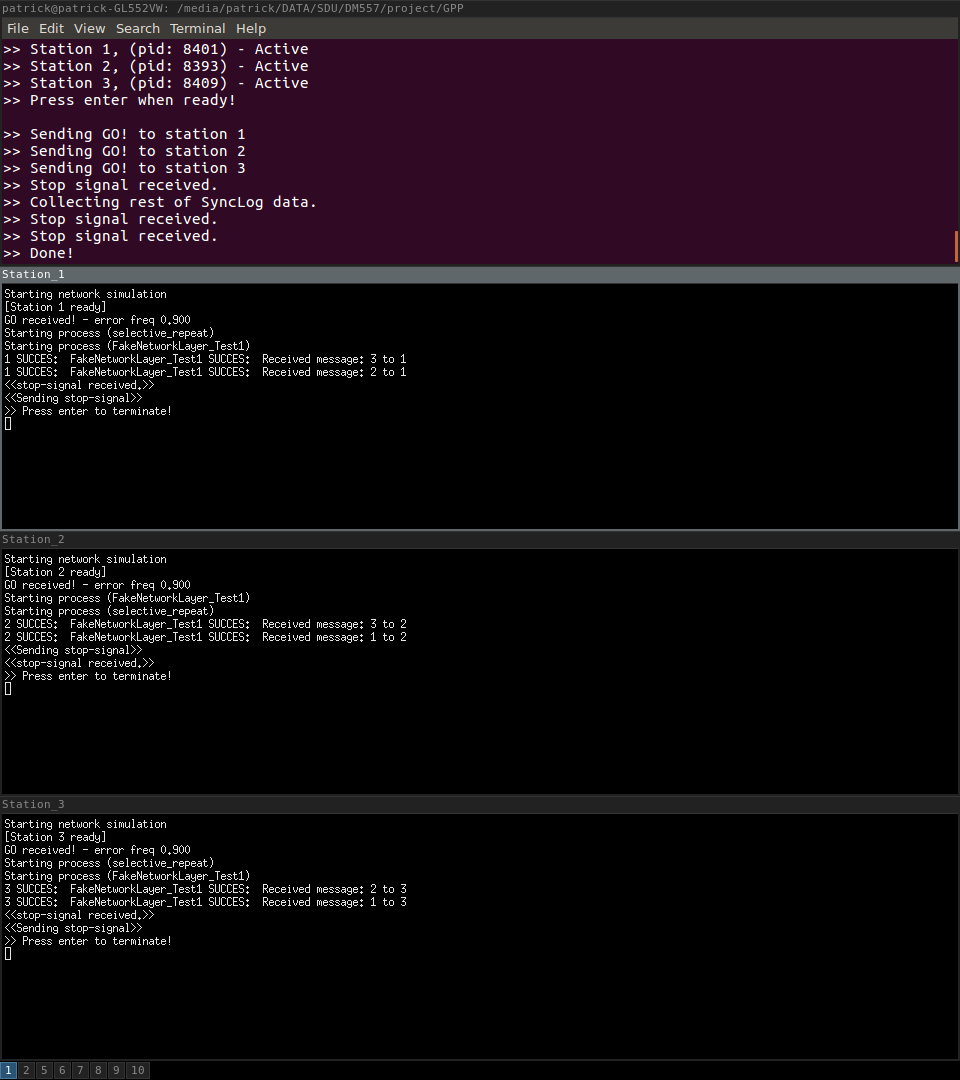
\includegraphics[width=0.6\textwidth]{Test1.png}
\caption{Test of three stations, each sending a message to the other two}
\label{fig:threestationtest}
\end{figure}




